\section{Memory Faults}
\label{sect:bg-faults}
Precise fault modeling is the key to designing efficient fault tests.  Fault models reflect real, specific defects in memory so high defect coverage and detection is strongly dependent on the quality of the fault model \cite{1327984}.  The following sections offer a brief description about the four classic types of faults \cite{Adams2003} that models are designed to detect.  

\subsection{Stuck-At Faults}
The most common type of memory fault occurs when the memory cell is locked into one state, either a “0” or “1”.  A defect free cell can be written to either state and, when read, will still contain the information previously written.  The stuck-at fault occurs when a state is written to the cell, but the subsequent reads return the only one state regardless of the previously written value.  Fig. 2 shows the state diagram for a stuck-at fault \cite{oldref-03}.
Another fault that can be classified as a stuck-at fault is the address decoder fault.  It is like the data stuck-at fault, but occurs on the address lines and leads to accessing wrong addresses, no addresses, or multiple addresses \cite{oldref-03}.

\subsection{Transitional Faults}
Similar to a stuck-at fault, the transition fault also locks into a single state, but has the characteristic of being in either state prior to the write.  The memory cell may contain “0” or “1” when powered on, but after a write, it cannot transition back.  The characteristic behavior of this fault is the memory can only written in one direction.  

\subsection{Coupling Faults}
There are numerous types of coupling faults, but they can be simply expressed as a cell affecting its neighboring cells and causing the neighbor to falsely transition or change state.  Coupling faults can be unidirectional or bi-directional.  In unidirectional coupling faults, one cell (aggressor cell) couples into another (victim cell), but the opposite does not occur.  A parasitic diode connection between the cells is a common cause of this behavior.  The bi-directional coupling fault occurs when pairs of cells can affect each other.  One way that this type of defect can occur is through bridging \cite{Adams2003}.  

\subsection{Neighborhood Pattern-Sensitive Fault (NPSF)}
\label{sec:npsf}
This fault model is in the class of coupling faults, but it is caused by particular patterns in neighboring cells rather than one specific cell.  The neighborhoods are usually defined as Type-1 or Type-2 neighborhoods \cite{1047051} as shown in Figure \ref{fig:npsftypes}.  Type-1 neighborhoods consist of five cells: one cell in center and four cells physically adjecent to the center cell.  In this configuration, the center cell is the base cell and the four adjecent cells are called the deleted neighborhood.  Type-2 neighborhoods consist of multiple cells where the base cell is in the center and deleted neighborhood is comprised of the cells within $m_1$ columns to the left, $m_2$ rows above, $m_3$ columns to the right and $m_4$ rows below the base cell.  This report will focus on Type-1 neighborhoods.

\begin{figure}[h!]
  \centering
  \begin{subfigure}[b]{0.4\textwidth}
    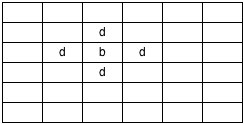
\includegraphics[width=\textwidth]{type1}
    \caption{Type-1 Neighborhood}
    \label{fig:type1}
  \end{subfigure}
  \begin{subfigure}[b]{0.4\textwidth}
    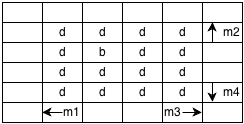
\includegraphics[width=\textwidth]{type2}
    \caption{Type-2 Neighborhood}
    \label{fig:type2}
  \end{subfigure}
  \caption{NPSF Neighborhoods \\
           b: base cell \\
           d: deleted neighborhood} 
           %$m_1$ = $m_2$ = 1; $m_3$ = $m_4$ = 2}
  \label{fig:npsftypes}
\end{figure}

Three classes of NPSF faults exist:
\begin{enumerate}
  \item Active NPSF (ANPSF): the base cell's contents change due to changes in the pattern of the deleted neighborhood.
  \item Passive NPSF (PNPSF): the base cell's contents cannot change due to specific pattern in the deleted neighborhood.
  \item Static NPSF (SNPSF): the base cell's contents are forced to a specific value because of the contents of the deleted neighborhood
\end{enumerate}

To test for all three classes of NPSF faults, all the combinations of values in the deleted cells and their transistions must be performed against the base cell.  To do this, a Eulerian Sequence is employed to generate the appropriate sequence of values in the neighborhood.  \cite{1675556} offers a proof of the Eulerian Sequence as a testing mechanism.  A 5-bit Eulerian Sequence is used as the Type-1 pattern.

To reudce the number of write operations to memory, multiple patterns can be written to memory simultaneously using either the tiling or two-group methods as shown in Figure \ref{fig:type1methods}.

\begin{figure}[h]
  \centering
  
\includegraphics[width=\textwidth]{placeholder}
  \caption{Type-1 with tiling method and two-group method}
  \label{fig:type1methods}
\end{figure}

In the tiling method, each tile is written to memory is such a way that none of the tiles overlap.  The two-group method is comprised to two checkerboard patterns that are overlaid is such a way that a base cell is in one checkerboard pattern while the deleted neighborhood is within the other checkerboard pattern.  This report will use the tiling method.
